\subsection*{Urzoni} % (fold)
\label{sub:urzoni}

\begin{multicols}{2}
	
Noční hra
V noci nás vzbudili křikem, že loď hoří. Museli jsme běhat s hrnečkem pro vodu a hasit ohně v lese. U ohně ale byli piráti a chytali nás. Potom, co jsme ohně uhasili, jsme si museli odnést svoji věc z celty, která byla za ohněma. Noční hra se mi moc líbyla.

\podpis{Čertisko}

JEDNOU JSME SE RÁNO PODÍVALI NA PROGRAM. A TAM ODCHOD NA MANÉVRY URZONI: HAHAHA ODCHOD NA MAÉVRY TO URČITĚ NEBUDEME ODCHÁZET NA MANÉVRY. BORŮVKY: ZABALÍME SE POTŘEBUJEME SPACÁK, KARIMATKU…

\podpis{SNĚH.}

Na posledním táboře jsem nebyl a to mě mrzí, a o to se víc těším na další.

\podpis{Polda}

Nejvíc mě se líbilo z etapky, jak sme odposlouchávali jsme kanibalové, bylo to strašně dobrý. Hlavně jak mluvili a kanibalové a taky jak chodili na obhlídku.

\podpis{HANUŠ}


JEDNA Z NEJLEPŠÍ HLÍDEK  NA TOMHLE TÁBOŘE
NA KONCI OBCHÁZIM S MOZARTEM A NAJEDNOU VEDLE ODPADOVKY “PRÁSK”. TAK JÁ: “MOZARTE, ŘVI!” MOZART: “TAK JO! PŘEPAD, PŘEPAD!

NEBO KONEC MANÉVRŮ:\\
VOSTROVCI SE MOJE ETAPKA S ČERTOVOU A SNĚHULÁKOVOU SKUPINKOU. TAK JSME ŠLI DO TÁBORA A RAFÍK SE TROCHU ZADEJCHAL A TAK JÁ, ČERT A SNĚHULÁK POČKALI S NÍM. PROTOŽE NA NÁS NEPOČKAL IKDYŽ JSME VOLALI. TAK JSME SE DOHODLI, ŽE SE JIM POMSTÍME. DOJDEME DO TÁBORA SPOLEČNĚ, TADY JE SKORO CELÝ DIALOG\\
JUMBO, KÁJA A MARUŠKA (J+K+M):\\
”URZONI DĚLEJTE!!\\
MY: NIC\\
J: “ČERTE, SNĚHULÁKU, DĚLEJTE!”\\
K: “PIŠKOTE, DĚLEJ!!”\\
MY: TICHO\\
J+K: “DĚLEJTE!”\\
MY: POMALU DEMO.\\
VYNOŘÍME SE NA LOUCE.\\
J:”SMČ, DĚLEJTE!!!!!!!!!!!”\\
K: “PIŠKOTE!”\\
DOJDEME KE KUCHYNI PLNĚ STEJNĚ.\\
J+K:”PROČ, JSTE NEŠLI RYCHLEJC!!!!”\\
PÍSKLE: “VÝTE, ŽE NEŠLO O TO, KDO DOJDE DŘÍV NEBO POZDĚJC.”

NOČKA S LIDOJEDAMA:\\
LIDOJED VYKAČ:”JÁ BÝT BLEDÁ TVÁŘ, TAK RYCHLE ZDRHAT”\\
VYZVĚDAČ KUJÓNKA: TICHO\\
LIDOJED VYKAČ: “JESTLI BLEDÁ TVÁŘ RYCHLE NEZDRHAT TAK JÁ ROZBÍT HUBU!”\\
PROSTĚ NEJLEPŠÍ TÁBOR!\\

\podpis{PIŠKOT, PIŠKOT, PIŠKOT...}

NEVÍM CO PSÁT NIC NEPÍŠU TAK AHOJ
AHOJ VŠICHNI NEVÍM CO PSÁT TAK RADŠI NIC NEPÍŠU TAK ZATÍM AHOJ!!! VÁŠ TELESHOPING ŠLÁGR! A TOSE VYPLATÍ.!?

\podpis{ASISTO}
\end{multicols}

\begin{center}

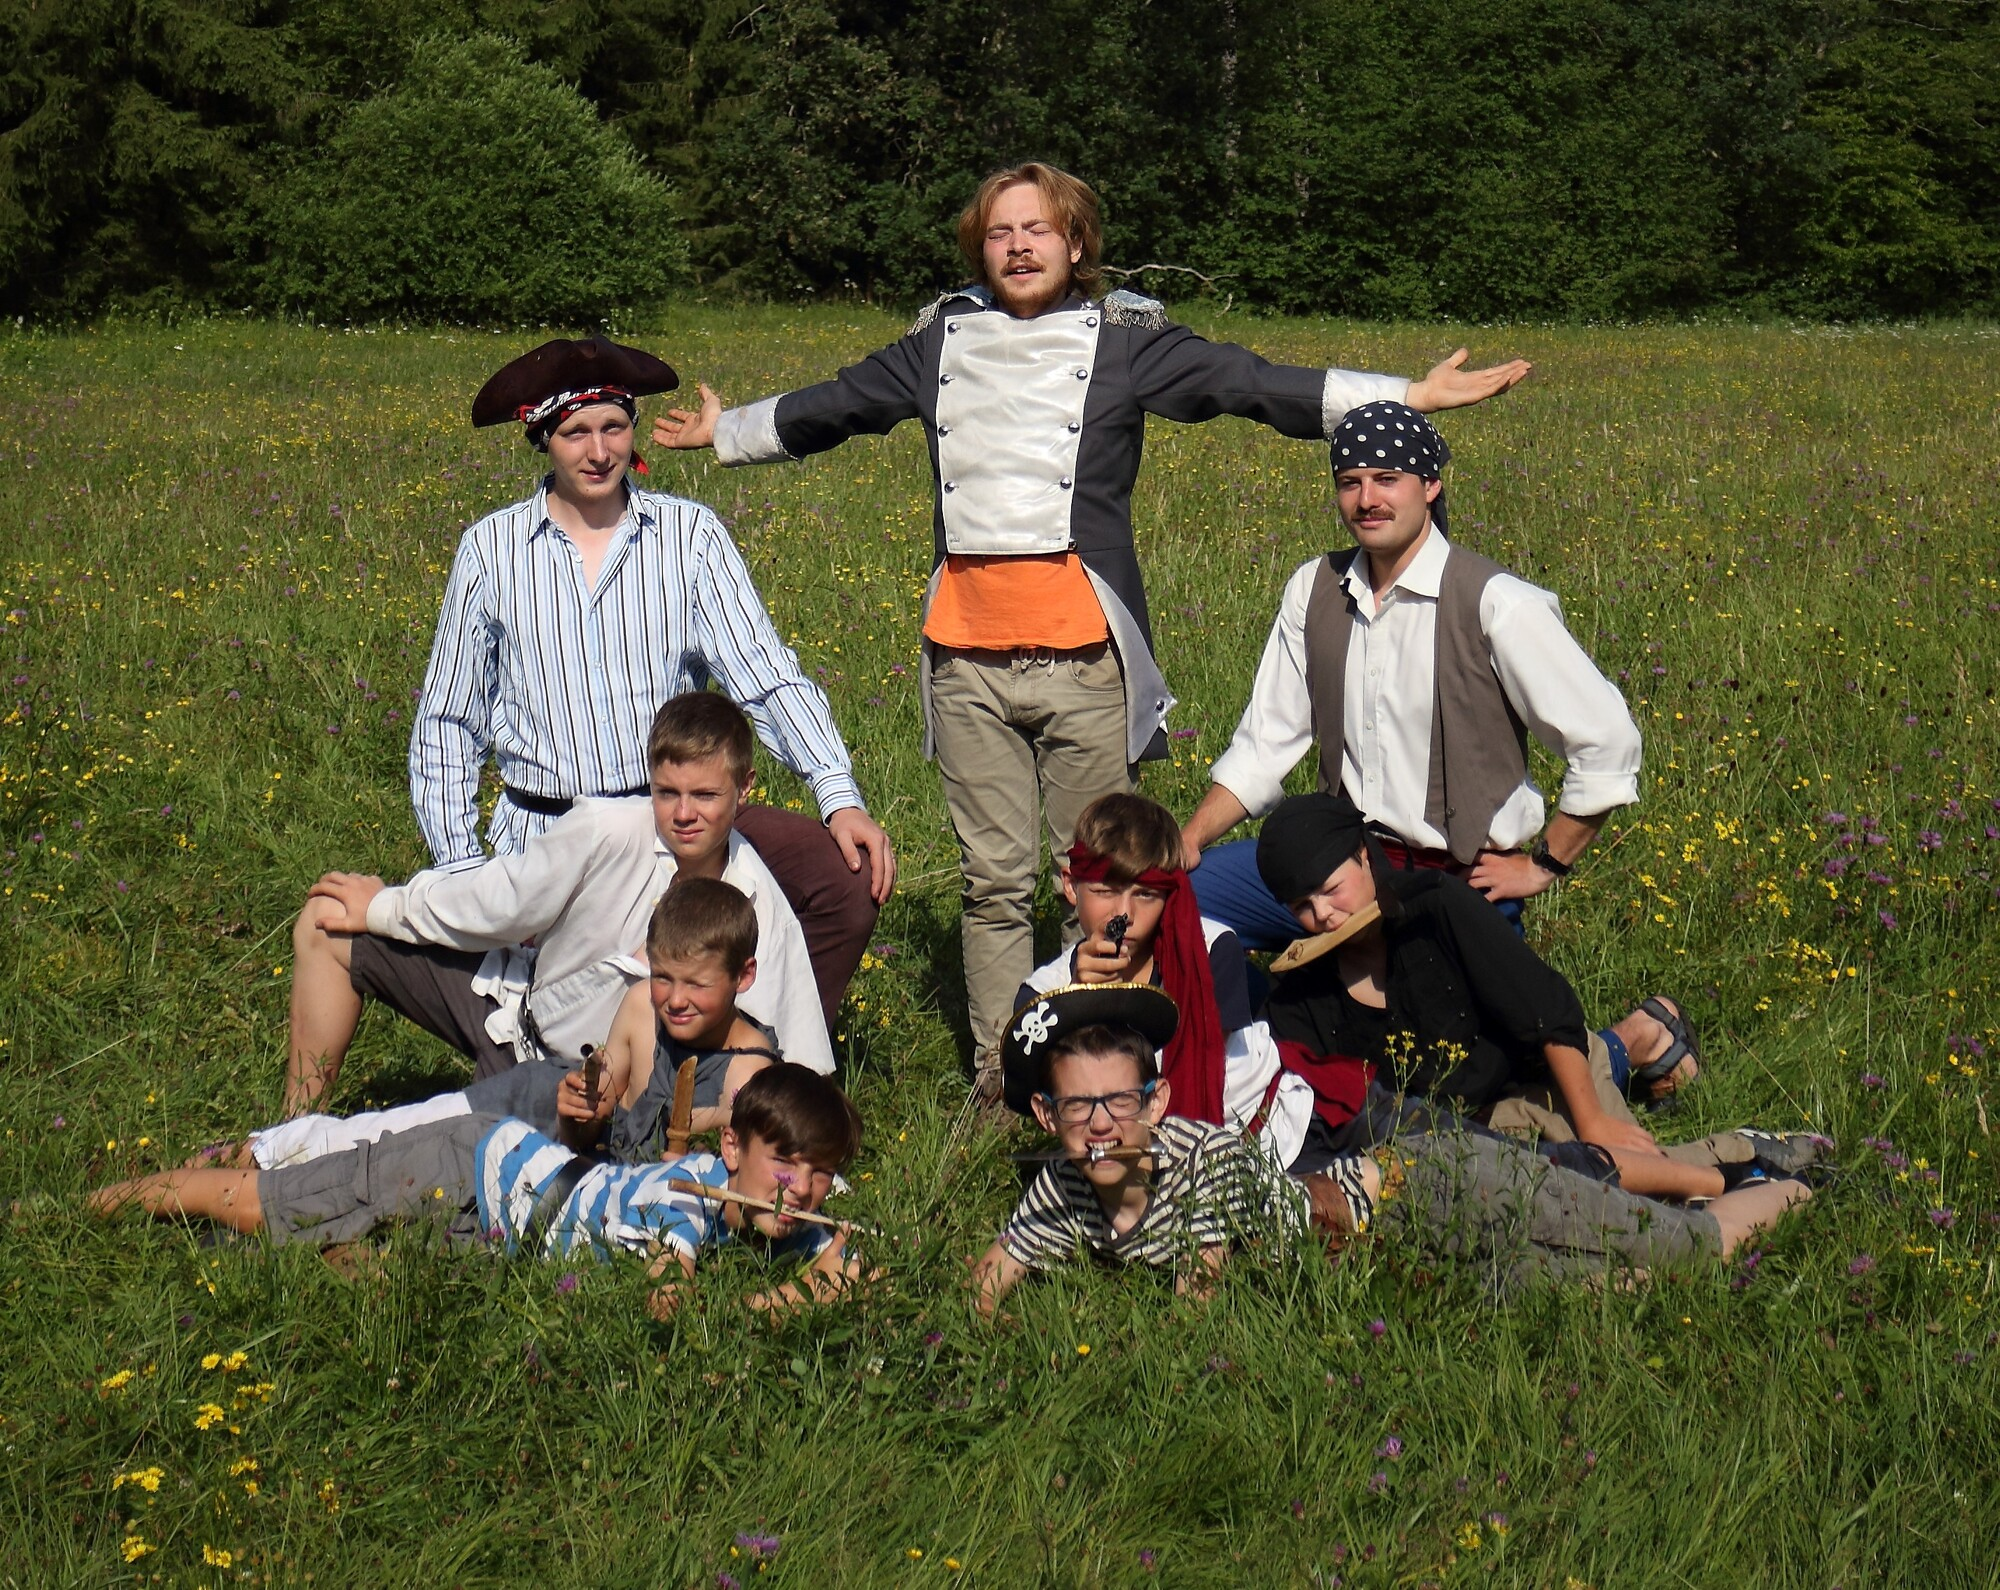
\includegraphics[width=10cm]{img/druziny/urzoni.JPG}

\end{center}

\clearpage

% subsection urzoni (end)
